\documentclass[12pt]{article}

%packages
%\usepackage{latexsym}
\usepackage{graphicx}
\usepackage{color}
\usepackage{amsmath}
\usepackage{dsfont}
\usepackage{placeins}
\usepackage{amssymb}
\usepackage{wasysym}
\usepackage{abstract}
\usepackage{hyperref}
\usepackage{etoolbox}
\usepackage{datetime}
\usepackage{xcolor}
\usepackage{alphalph}
\settimeformat{ampmtime}

%\usepackage{pstricks,pst-node,pst-tree}

%\usepackage{algpseudocode}
%\usepackage{amsthm}
%\usepackage{hyperref}
%\usepackage{mathrsfs}
%\usepackage{amsfonts}
%\usepackage{bbding}
%\usepackage{listings}
%\usepackage{appendix}
\usepackage[margin=1in]{geometry}
%\geometry{papersize={8.5in,11in},total={6.5in,9in}}
%\usepackage{cancel}
%\usepackage{algorithmic, algorithm}

\makeatletter
\def\maxwidth{ %
  \ifdim\Gin@nat@width>\linewidth
    \linewidth
  \else
    \Gin@nat@width
  \fi
}
\makeatother

\definecolor{fgcolor}{rgb}{0.345, 0.345, 0.345}
\newcommand{\hlnum}[1]{\textcolor[rgb]{0.686,0.059,0.569}{#1}}%
\newcommand{\hlstr}[1]{\textcolor[rgb]{0.192,0.494,0.8}{#1}}%
\newcommand{\hlcom}[1]{\textcolor[rgb]{0.678,0.584,0.686}{\textit{#1}}}%
\newcommand{\hlopt}[1]{\textcolor[rgb]{0,0,0}{#1}}%
\newcommand{\hlstd}[1]{\textcolor[rgb]{0.345,0.345,0.345}{#1}}%
\newcommand{\hlkwa}[1]{\textcolor[rgb]{0.161,0.373,0.58}{\textbf{#1}}}%
\newcommand{\hlkwb}[1]{\textcolor[rgb]{0.69,0.353,0.396}{#1}}%
\newcommand{\hlkwc}[1]{\textcolor[rgb]{0.333,0.667,0.333}{#1}}%
\newcommand{\hlkwd}[1]{\textcolor[rgb]{0.737,0.353,0.396}{\textbf{#1}}}%

\usepackage{framed}
\makeatletter
\newenvironment{kframe}{%
 \def\at@end@of@kframe{}%
 \ifinner\ifhmode%
  \def\at@end@of@kframe{\end{minipage}}%
  \begin{minipage}{\columnwidth}%
 \fi\fi%
 \def\FrameCommand##1{\hskip\@totalleftmargin \hskip-\fboxsep
 \colorbox{shadecolor}{##1}\hskip-\fboxsep
     % There is no \\@totalrightmargin, so:
     \hskip-\linewidth \hskip-\@totalleftmargin \hskip\columnwidth}%
 \MakeFramed {\advance\hsize-\width
   \@totalleftmargin\z@ \linewidth\hsize
   \@setminipage}}%
 {\par\unskip\endMakeFramed%
 \at@end@of@kframe}
\makeatother

\definecolor{shadecolor}{rgb}{.77, .77, .77}
\definecolor{messagecolor}{rgb}{0, 0, 0}
\definecolor{warningcolor}{rgb}{1, 0, 1}
\definecolor{errorcolor}{rgb}{1, 0, 0}
\newenvironment{knitrout}{}{} % an empty environment to be redefined in TeX

\usepackage{alltt}
\usepackage[T1]{fontenc}

\newcommand{\qu}[1]{``#1''}
\newcounter{probnum}
\setcounter{probnum}{1}

%create definition to allow local margin changes
\def\changemargin#1#2{\list{}{\rightmargin#2\leftmargin#1}\item[]}
\let\endchangemargin=\endlist 

%allow equations to span multiple pages
\allowdisplaybreaks

%define colors and color typesetting conveniences
\definecolor{gray}{rgb}{0.5,0.5,0.5}
\definecolor{black}{rgb}{0,0,0}
\definecolor{white}{rgb}{1,1,1}
\definecolor{blue}{rgb}{0.5,0.5,1}
\newcommand{\inblue}[1]{\color{blue}#1 \color{black}}
\definecolor{green}{rgb}{0.133,0.545,0.133}
\newcommand{\ingreen}[1]{\color{green}#1 \color{black}}
\definecolor{yellow}{rgb}{1,1,0}
\newcommand{\inyellow}[1]{\color{yellow}#1 \color{black}}
\definecolor{orange}{rgb}{0.9,0.649,0}
\newcommand{\inorange}[1]{\color{orange}#1 \color{black}}
\definecolor{red}{rgb}{1,0.133,0.133}
\newcommand{\inred}[1]{\color{red}#1 \color{black}}
\definecolor{purple}{rgb}{0.58,0,0.827}
\newcommand{\inpurple}[1]{\color{purple}#1 \color{black}}
\definecolor{backgcode}{rgb}{0.97,0.97,0.8}
\definecolor{Brown}{cmyk}{0,0.81,1,0.60}
\definecolor{OliveGreen}{cmyk}{0.64,0,0.95,0.40}
\definecolor{CadetBlue}{cmyk}{0.62,0.57,0.23,0}

%define new math operators
\DeclareMathOperator*{\argmax}{arg\,max~}
\DeclareMathOperator*{\argmin}{arg\,min~}
\DeclareMathOperator*{\argsup}{arg\,sup~}
\DeclareMathOperator*{\arginf}{arg\,inf~}
\DeclareMathOperator*{\convolution}{\text{\Huge{$\ast$}}}
\newcommand{\infconv}[2]{\convolution^\infty_{#1 = 1} #2}
%true functions

%%%% GENERAL SHORTCUTS

%shortcuts for pure typesetting conveniences
\newcommand{\bv}[1]{\boldsymbol{#1}}

%shortcuts for compound constants
\newcommand{\BetaDistrConst}{\dfrac{\Gamma(\alpha + \beta)}{\Gamma(\alpha)\Gamma(\beta)}}
\newcommand{\NormDistrConst}{\dfrac{1}{\sqrt{2\pi\sigma^2}}}

%shortcuts for conventional symbols
\newcommand{\tsq}{\tau^2}
\newcommand{\tsqh}{\hat{\tau}^2}
\newcommand{\sigsq}{\sigma^2}
\newcommand{\sigsqsq}{\parens{\sigma^2}^2}
\newcommand{\sigsqovern}{\dfrac{\sigsq}{n}}
\newcommand{\tausq}{\tau^2}
\newcommand{\tausqalpha}{\tau^2_\alpha}
\newcommand{\tausqbeta}{\tau^2_\beta}
\newcommand{\tausqsigma}{\tau^2_\sigma}
\newcommand{\betasq}{\beta^2}
\newcommand{\sigsqvec}{\bv{\sigma}^2}
\newcommand{\sigsqhat}{\hat{\sigma}^2}
\newcommand{\sigsqhatmlebayes}{\sigsqhat_{\text{Bayes, MLE}}}
\newcommand{\sigsqhatmle}[1]{\sigsqhat_{#1, \text{MLE}}}
\newcommand{\bSigma}{\bv{\Sigma}}
\newcommand{\bSigmainv}{\bSigma^{-1}}
\newcommand{\thetavec}{\bv{\theta}}
\newcommand{\thetahat}{\hat{\theta}}
\newcommand{\thetahatmle}{\hat{\theta}_{\mathrm{MLE}}}
\newcommand{\thetavechatmle}{\hat{\thetavec}_{\mathrm{MLE}}}
\newcommand{\muhat}{\hat{\mu}}
\newcommand{\musq}{\mu^2}
\newcommand{\muvec}{\bv{\mu}}
\newcommand{\muhatmle}{\muhat_{\text{MLE}}}
\newcommand{\lambdahat}{\hat{\lambda}}
\newcommand{\lambdahatmle}{\lambdahat_{\text{MLE}}}
\newcommand{\etavec}{\bv{\eta}}
\newcommand{\alphavec}{\bv{\alpha}}
\newcommand{\minimaxdec}{\delta^*_{\mathrm{mm}}}
\newcommand{\ybar}{\bar{y}}
\newcommand{\xbar}{\bar{x}}
\newcommand{\Xbar}{\bar{X}}
\newcommand{\phat}{\hat{p}}
\newcommand{\Phat}{\hat{P}}
\newcommand{\Zbar}{\bar{Z}}
\newcommand{\iid}{~{\buildrel iid \over \sim}~}
\newcommand{\inddist}{~{\buildrel ind \over \sim}~}
\newcommand{\approxdist}{~{\buildrel approx \over \sim}~}
\newcommand{\equalsindist}{~{\buildrel d \over =}~}
\newcommand{\loglik}[1]{\ell\parens{#1}}
\newcommand{\thetahatkminone}{\thetahat^{(k-1)}}
\newcommand{\thetahatkplusone}{\thetahat^{(k+1)}}
\newcommand{\thetahatk}{\thetahat^{(k)}}
\newcommand{\half}{\frac{1}{2}}
\newcommand{\third}{\frac{1}{3}}
\newcommand{\twothirds}{\frac{2}{3}}
\newcommand{\fourth}{\frac{1}{4}}
\newcommand{\fifth}{\frac{1}{5}}
\newcommand{\sixth}{\frac{1}{6}}

%shortcuts for vector and matrix notation
\newcommand{\A}{\bv{A}}
\newcommand{\At}{\A^T}
\newcommand{\Ainv}{\inverse{\A}}
\newcommand{\B}{\bv{B}}
\newcommand{\K}{\bv{K}}
\newcommand{\Kt}{\K^T}
\newcommand{\Kinv}{\inverse{K}}
\newcommand{\Kinvt}{(\Kinv)^T}
\newcommand{\M}{\bv{M}}
\newcommand{\Bt}{\B^T}
\newcommand{\Q}{\bv{Q}}
\newcommand{\Qt}{\Q^T}
\newcommand{\R}{\bv{R}}
\newcommand{\Rt}{\R^T}
\newcommand{\Z}{\bv{Z}}
\newcommand{\X}{\bv{X}}
\newcommand{\Xsub}{\X_{\text{(sub)}}}
\newcommand{\Xsubadj}{\X_{\text{(sub,adj)}}}
\newcommand{\I}{\bv{I}}
\newcommand{\Y}{\bv{Y}}
\newcommand{\sigsqI}{\sigsq\I}
\renewcommand{\P}{\bv{P}}
\newcommand{\Psub}{\P_{\text{(sub)}}}
\newcommand{\Pt}{\P^T}
\newcommand{\Pii}{P_{ii}}
\newcommand{\Pij}{P_{ij}}
\newcommand{\IminP}{(\I-\P)}
\newcommand{\Xt}{\bv{X}^T}
\newcommand{\XtX}{\Xt\X}
\newcommand{\XtXinv}{\parens{\Xt\X}^{-1}}
\newcommand{\XtXinvXt}{\XtXinv\Xt}
\newcommand{\XXtXinvXt}{\X\XtXinvXt}
\newcommand{\x}{\bv{x}}
\newcommand{\onevec}{\bv{1}}
\newcommand{\oneton}{1, \ldots, n}
\newcommand{\yoneton}{y_1, \ldots, y_n}
\newcommand{\yonetonorder}{y_{(1)}, \ldots, y_{(n)}}
\newcommand{\Yoneton}{Y_1, \ldots, Y_n}
\newcommand{\iinoneton}{i \in \braces{\oneton}}
\newcommand{\onetom}{1, \ldots, m}
\newcommand{\jinonetom}{j \in \braces{\onetom}}
\newcommand{\xoneton}{x_1, \ldots, x_n}
\newcommand{\Xoneton}{X_1, \ldots, X_n}
\newcommand{\xt}{\x^T}
\newcommand{\y}{\bv{y}}
\newcommand{\yt}{\y^T}
\renewcommand{\c}{\bv{c}}
\newcommand{\ct}{\c^T}
\newcommand{\tstar}{\bv{t}^*}
\renewcommand{\u}{\bv{u}}
\renewcommand{\v}{\bv{v}}
\renewcommand{\a}{\bv{a}}
\newcommand{\s}{\bv{s}}
\newcommand{\yadj}{\y_{\text{(adj)}}}
\newcommand{\xjadj}{\x_{j\text{(adj)}}}
\newcommand{\xjadjM}{\x_{j \perp M}}
\newcommand{\yhat}{\hat{\y}}
\newcommand{\yhatsub}{\yhat_{\text{(sub)}}}
\newcommand{\yhatstar}{\yhat^*}
\newcommand{\yhatstarnew}{\yhatstar_{\text{new}}}
\newcommand{\z}{\bv{z}}
\newcommand{\zt}{\z^T}
\newcommand{\bb}{\bv{b}}
\newcommand{\bbt}{\bb^T}
\newcommand{\bbeta}{\bv{\beta}}
\newcommand{\beps}{\bv{\epsilon}}
\newcommand{\bepst}{\beps^T}
\newcommand{\e}{\bv{e}}
\newcommand{\Mofy}{\M(\y)}
\newcommand{\KofAlpha}{K(\alpha)}
\newcommand{\ellset}{\mathcal{L}}
\newcommand{\oneminalph}{1-\alpha}
\newcommand{\SSE}{\text{SSE}}
\newcommand{\SSEsub}{\text{SSE}_{\text{(sub)}}}
\newcommand{\MSE}{\text{MSE}}
\newcommand{\RMSE}{\text{RMSE}}
\newcommand{\SSR}{\text{SSR}}
\newcommand{\SST}{\text{SST}}
\newcommand{\JSest}{\delta_{\text{JS}}(\x)}
\newcommand{\Bayesest}{\delta_{\text{Bayes}}(\x)}
\newcommand{\EmpBayesest}{\delta_{\text{EmpBayes}}(\x)}
\newcommand{\BLUPest}{\delta_{\text{BLUP}}}
\newcommand{\MLEest}[1]{\hat{#1}_{\text{MLE}}}

%shortcuts for Linear Algebra stuff (i.e. vectors and matrices)
\newcommand{\twovec}[2]{\bracks{\begin{array}{c} #1 \\ #2 \end{array}}}
\newcommand{\threevec}[3]{\bracks{\begin{array}{c} #1 \\ #2 \\ #3 \end{array}}}
\newcommand{\fivevec}[5]{\bracks{\begin{array}{c} #1 \\ #2 \\ #3 \\ #4 \\ #5 \end{array}}}
\newcommand{\twobytwomat}[4]{\bracks{\begin{array}{cc} #1 & #2 \\ #3 & #4 \end{array}}}
\newcommand{\threebytwomat}[6]{\bracks{\begin{array}{cc} #1 & #2 \\ #3 & #4 \\ #5 & #6 \end{array}}}

%shortcuts for conventional compound symbols
\newcommand{\thetainthetas}{\theta \in \Theta}
\newcommand{\reals}{\mathbb{R}}
\newcommand{\complexes}{\mathbb{C}}
\newcommand{\rationals}{\mathbb{Q}}
\newcommand{\integers}{\mathbb{Z}}
\newcommand{\naturals}{\mathbb{N}}
\newcommand{\forallninN}{~~\forall n \in \naturals}
\newcommand{\forallxinN}[1]{~~\forall #1 \in \reals}
\newcommand{\matrixdims}[2]{\in \reals^{\,#1 \times #2}}
\newcommand{\inRn}[1]{\in \reals^{\,#1}}
\newcommand{\mathimplies}{\quad\Rightarrow\quad}
\newcommand{\mathlogicequiv}{\quad\Leftrightarrow\quad}
\newcommand{\eqncomment}[1]{\quad \text{(#1)}}
\newcommand{\limitn}{\lim_{n \rightarrow \infty}}
\newcommand{\limitN}{\lim_{N \rightarrow \infty}}
\newcommand{\limitd}{\lim_{d \rightarrow \infty}}
\newcommand{\limitt}{\lim_{t \rightarrow \infty}}
\newcommand{\limitsupn}{\limsup_{n \rightarrow \infty}~}
\newcommand{\limitinfn}{\liminf_{n \rightarrow \infty}~}
\newcommand{\limitk}{\lim_{k \rightarrow \infty}}
\newcommand{\limsupn}{\limsup_{n \rightarrow \infty}}
\newcommand{\limsupk}{\limsup_{k \rightarrow \infty}}
\newcommand{\floor}[1]{\left\lfloor #1 \right\rfloor}
\newcommand{\ceil}[1]{\left\lceil #1 \right\rceil}

%shortcuts for environments
\newcommand{\beqn}{\vspace{-0.25cm}\begin{eqnarray*}}
\newcommand{\eeqn}{\end{eqnarray*}}
\newcommand{\bneqn}{\vspace{-0.25cm}\begin{eqnarray}}
\newcommand{\eneqn}{\end{eqnarray}}

%shortcuts for mini environments
\newcommand{\parens}[1]{\left(#1\right)}
\newcommand{\squared}[1]{\parens{#1}^2}
\newcommand{\tothepow}[2]{\parens{#1}^{#2}}
\newcommand{\prob}[1]{\mathbb{P}\parens{#1}}
\newcommand{\cprob}[2]{\prob{#1~|~#2}}
\newcommand{\littleo}[1]{o\parens{#1}}
\newcommand{\bigo}[1]{O\parens{#1}}
\newcommand{\Lp}[1]{\mathbb{L}^{#1}}
\renewcommand{\arcsin}[1]{\text{arcsin}\parens{#1}}
\newcommand{\prodonen}[2]{\bracks{\prod_{#1=1}^n #2}}
\newcommand{\mysum}[4]{\sum_{#1=#2}^{#3} #4}
\newcommand{\sumonen}[2]{\sum_{#1=1}^n #2}
\newcommand{\infsum}[2]{\sum_{#1=1}^\infty #2}
\newcommand{\infprod}[2]{\prod_{#1=1}^\infty #2}
\newcommand{\infunion}[2]{\bigcup_{#1=1}^\infty #2}
\newcommand{\infinter}[2]{\bigcap_{#1=1}^\infty #2}
\newcommand{\infintegral}[2]{\int^\infty_{-\infty} #2 ~\text{d}#1}
\newcommand{\supthetas}[1]{\sup_{\thetainthetas}\braces{#1}}
\newcommand{\bracks}[1]{\left[#1\right]}
\newcommand{\braces}[1]{\left\{#1\right\}}
\newcommand{\angbraces}[1]{\left<#1\right>}
\newcommand{\set}[1]{\left\{#1\right\}}
\newcommand{\abss}[1]{\left|#1\right|}
\newcommand{\norm}[1]{\left|\left|#1\right|\right|}
\newcommand{\normsq}[1]{\norm{#1}^2}
\newcommand{\inverse}[1]{\parens{#1}^{-1}}
\newcommand{\rowof}[2]{\parens{#1}_{#2\cdot}}

%shortcuts for functionals
\newcommand{\realcomp}[1]{\text{Re}\bracks{#1}}
\newcommand{\imagcomp}[1]{\text{Im}\bracks{#1}}
\newcommand{\range}[1]{\text{range}\bracks{#1}}
\newcommand{\colsp}[1]{\text{colsp}\bracks{#1}}
\newcommand{\rowsp}[1]{\text{rowsp}\bracks{#1}}
\newcommand{\tr}[1]{\text{tr}\bracks{#1}}
\newcommand{\rank}[1]{\text{rank}\bracks{#1}}
\newcommand{\proj}[2]{\text{Proj}_{#1}\bracks{#2}}
\newcommand{\projcolspX}[1]{\text{Proj}_{\colsp{\X}}\bracks{#1}}
\newcommand{\median}[1]{\text{median}\bracks{#1}}
\newcommand{\mean}[1]{\text{mean}\bracks{#1}}
\newcommand{\dime}[1]{\text{dim}\bracks{#1}}
\renewcommand{\det}[1]{\text{det}\bracks{#1}}
\newcommand{\expe}[1]{\mathbb{E}\bracks{#1}}
\newcommand{\expeabs}[1]{\expe{\abss{#1}}}
\newcommand{\expesub}[2]{\mathbb{E}_{#1}\bracks{#2}}
\newcommand{\indic}[1]{\mathds{1}_{#1}}
\newcommand{\var}[1]{\mathbb{V}\text{ar}\bracks{#1}}
\newcommand{\cov}[2]{\mathbb{C}\text{ov}\bracks{#1, #2}}
\newcommand{\corr}[2]{\text{Corr}\bracks{#1, #2}}
\newcommand{\se}[1]{\mathbb{S}\text{E}\bracks{#1}}
\newcommand{\seest}[1]{\hat{\text{SE}}\bracks{#1}}
\newcommand{\bias}[1]{\text{Bias}\bracks{#1}}
\newcommand{\derivop}[2]{\dfrac{\text{d}}{\text{d} #1}\bracks{#2}}
\newcommand{\partialop}[2]{\dfrac{\partial}{\partial #1}\bracks{#2}}
\newcommand{\secpartialop}[2]{\dfrac{\partial^2}{\partial #1^2}\bracks{#2}}
\newcommand{\mixpartialop}[3]{\dfrac{\partial^2}{\partial #1 \partial #2}\bracks{#3}}

%shortcuts for functions
\renewcommand{\exp}[1]{\mathrm{exp}\parens{#1}}
\renewcommand{\cos}[1]{\text{cos}\parens{#1}}
\renewcommand{\sin}[1]{\text{sin}\parens{#1}}
\newcommand{\sign}[1]{\text{sign}\parens{#1}}
\newcommand{\are}[1]{\mathrm{ARE}\parens{#1}}
\newcommand{\natlog}[1]{\ln\parens{#1}}
\newcommand{\oneover}[1]{\frac{1}{#1}}
\newcommand{\overtwo}[1]{\frac{#1}{2}}
\newcommand{\overn}[1]{\frac{#1}{n}}
\newcommand{\oneoversqrt}[1]{\oneover{\sqrt{#1}}}
\newcommand{\sqd}[1]{\parens{#1}^2}
\newcommand{\loss}[1]{\ell\parens{\theta, #1}}
\newcommand{\losstwo}[2]{\ell\parens{#1, #2}}
\newcommand{\cf}{\phi(t)}

%English language specific shortcuts
\newcommand{\ie}{\textit{i.e.} }
\newcommand{\AKA}{\textit{AKA} }
\renewcommand{\iff}{\textit{iff}}
\newcommand{\eg}{\textit{e.g.} }
\newcommand{\st}{\textit{s.t.} }
\newcommand{\wrt}{\textit{w.r.t.} }
\newcommand{\mathst}{~~\text{\st}~~}
\newcommand{\mathand}{~~\text{and}~~}
\newcommand{\ala}{\textit{a la} }
\newcommand{\ppp}{posterior predictive p-value}
\newcommand{\dd}{dataset-to-dataset}

%shortcuts for distribution titles
\newcommand{\logistic}[2]{\mathrm{Logistic}\parens{#1,\,#2}}
\newcommand{\bernoulli}[1]{\mathrm{Bernoulli}\parens{#1}}
\newcommand{\betanot}[2]{\mathrm{Beta}\parens{#1,\,#2}}
\newcommand{\stdbetanot}{\betanot{\alpha}{\beta}}
\newcommand{\multnormnot}[3]{\mathcal{N}_{#1}\parens{#2,\,#3}}
\newcommand{\normnot}[2]{\mathcal{N}\parens{#1,\,#2}}
\newcommand{\classicnormnot}{\normnot{\mu}{\sigsq}}
\newcommand{\stdnormnot}{\normnot{0}{1}}
\newcommand{\uniformdiscrete}[1]{\mathrm{Uniform}\parens{\braces{#1}}}
\newcommand{\uniform}[2]{\mathrm{U}\parens{#1,\,#2}}
\newcommand{\stduniform}{\uniform{0}{1}}
\newcommand{\geometric}[1]{\mathrm{Geometric}\parens{#1}}
\newcommand{\hypergeometric}[3]{\mathrm{Hypergeometric}\parens{#1,\,#2,\,#3}}
\newcommand{\exponential}[1]{\mathrm{Exp}\parens{#1}}
\newcommand{\gammadist}[2]{\mathrm{Gamma}\parens{#1, #2}}
\newcommand{\poisson}[1]{\mathrm{Poisson}\parens{#1}}
\newcommand{\binomial}[2]{\mathrm{Binomial}\parens{#1,\,#2}}
\newcommand{\negbin}[2]{\mathrm{NegBin}\parens{#1,\,#2}}
\newcommand{\rayleigh}[1]{\mathrm{Rayleigh}\parens{#1}}
\newcommand{\multinomial}[2]{\mathrm{Multinomial}\parens{#1,\,#2}}
\newcommand{\gammanot}[2]{\mathrm{Gamma}\parens{#1,\,#2}}
\newcommand{\cauchynot}[2]{\text{Cauchy}\parens{#1,\,#2}}
\newcommand{\invchisqnot}[1]{\text{Inv}\chisq{#1}}
\newcommand{\invscaledchisqnot}[2]{\text{ScaledInv}\ncchisq{#1}{#2}}
\newcommand{\invgammanot}[2]{\text{InvGamma}\parens{#1,\,#2}}
\newcommand{\chisq}[1]{\chi^2_{#1}}
\newcommand{\ncchisq}[2]{\chi^2_{#1}\parens{#2}}
\newcommand{\ncF}[3]{F_{#1,#2}\parens{#3}}

%shortcuts for PDF's of common distributions
\newcommand{\logisticpdf}[3]{\oneover{#3}\dfrac{\exp{-\dfrac{#1 - #2}{#3}}}{\parens{1+\exp{-\dfrac{#1 - #2}{#3}}}^2}}
\newcommand{\betapdf}[3]{\dfrac{\Gamma(#2 + #3)}{\Gamma(#2)\Gamma(#3)}#1^{#2-1} (1-#1)^{#3-1}}
\newcommand{\normpdf}[3]{\frac{1}{\sqrt{2\pi#3}}\exp{-\frac{1}{2#3}(#1 - #2)^2}}
\newcommand{\normpdfvarone}[2]{\dfrac{1}{\sqrt{2\pi}}e^{-\half(#1 - #2)^2}}
\newcommand{\chisqpdf}[2]{\dfrac{1}{2^{#2/2}\Gamma(#2/2)}\; {#1}^{#2/2-1} e^{-#1/2}}
\newcommand{\invchisqpdf}[2]{\dfrac{2^{-\overtwo{#1}}}{\Gamma(#2/2)}\,{#1}^{-\overtwo{#2}-1}  e^{-\oneover{2 #1}}}
\newcommand{\exponentialpdf}[2]{#2\exp{-#2#1}}
\newcommand{\poissonpdf}[2]{\dfrac{e^{-#1} #1^{#2}}{#2!}}
\newcommand{\binomialpdf}[3]{\binom{#2}{#1}#3^{#1}(1-#3)^{#2-#1}}
\newcommand{\rayleighpdf}[2]{\dfrac{#1}{#2^2}\exp{-\dfrac{#1^2}{2 #2^2}}}
\newcommand{\gammapdf}[3]{\dfrac{#3^#2}{\Gamma\parens{#2}}#1^{#2-1}\exp{-#3 #1}}
\newcommand{\cauchypdf}[3]{\oneover{\pi} \dfrac{#3}{\parens{#1-#2}^2 + #3^2}}
\newcommand{\Gammaf}[1]{\Gamma\parens{#1}}

%shortcuts for miscellaneous typesetting conveniences
\newcommand{\notesref}[1]{\marginpar{\color{gray}\tt #1\color{black}}}

%%%% DOMAIN-SPECIFIC SHORTCUTS

%Real analysis related shortcuts
\newcommand{\zeroonecl}{\bracks{0,1}}
\newcommand{\forallepsgrzero}{\forall \epsilon > 0~~}
\newcommand{\lessthaneps}{< \epsilon}
\newcommand{\fraccomp}[1]{\text{frac}\bracks{#1}}

%Bayesian related shortcuts
\newcommand{\yrep}{y^{\text{rep}}}
\newcommand{\yrepisq}{(\yrep_i)^2}
\newcommand{\yrepvec}{\bv{y}^{\text{rep}}}


%Probability shortcuts
\newcommand{\SigField}{\mathcal{F}}
\newcommand{\ProbMap}{\mathcal{P}}
\newcommand{\probtrinity}{\parens{\Omega, \SigField, \ProbMap}}
\newcommand{\convp}{~{\buildrel p \over \rightarrow}~}
\newcommand{\convLp}[1]{~{\buildrel \Lp{#1} \over \rightarrow}~}
\newcommand{\nconvp}{~{\buildrel p \over \nrightarrow}~}
\newcommand{\convae}{~{\buildrel a.e. \over \longrightarrow}~}
\newcommand{\convau}{~{\buildrel a.u. \over \longrightarrow}~}
\newcommand{\nconvau}{~{\buildrel a.u. \over \nrightarrow}~}
\newcommand{\nconvae}{~{\buildrel a.e. \over \nrightarrow}~}
\newcommand{\convd}{~{\buildrel \mathcal{D} \over \rightarrow}~}
\newcommand{\nconvd}{~{\buildrel \mathcal{D} \over \nrightarrow}~}
\newcommand{\withprob}{~~\text{w.p.}~~}
\newcommand{\io}{~~\text{i.o.}}

\newcommand{\Acl}{\bar{A}}
\newcommand{\ENcl}{\bar{E}_N}
\newcommand{\diam}[1]{\text{diam}\parens{#1}}

\newcommand{\taua}{\tau_a}

\newcommand{\myint}[4]{\int_{#2}^{#3} #4 \,\text{d}#1}
\newcommand{\laplacet}[1]{\mathscr{L}\bracks{#1}}
\newcommand{\laplaceinvt}[1]{\mathscr{L}^{-1}\bracks{#1}}
\renewcommand{\min}[1]{\text{min}\braces{#1}}
\renewcommand{\max}[1]{\text{max}\braces{#1}}

\newcommand{\Vbar}[1]{\bar{V}\parens{#1}}
\newcommand{\expnegrtau}{\exp{-r\tau}}

%%% problem typesetting
\newcommand{\problem}{\noindent \colorbox{black}{{\color{yellow} \large{\textsf{\textbf{Problem \arabic{probnum}}}}~}} \addtocounter{probnum}{1} \vspace{0.2cm} \\ }

\newcommand{\easysubproblem}{\ingreen{\item} [easy] }
\newcommand{\intermediatesubproblem}{\inorange{\item} [harder] }
\newcommand{\hardsubproblem}{\inred{\item} [difficult] }
\newcommand{\extracreditsubproblem}{\inpurple{\item} [E.C.] }

\makeatletter
\newalphalph{\alphmult}[mult]{\@alph}{26}
\renewcommand{\labelenumi}{(\alphmult{\value{enumi}})}

\newcommand{\support}[1]{\text{Supp}\bracks{#1}}
\newcommand{\mode}[1]{\text{Mode}\bracks{#1}}
\newcommand{\IQR}[1]{\text{IQR}\bracks{#1}}
\newcommand{\quantile}[2]{\text{Quantile}\bracks{#1,\,#2}}


\newtoggle{professormode}
\toggletrue{professormode} %STUDENTS: DELETE or COMMENT this line



\title{MATH 241 Fall 2017 Homework \#4}

\author{Professor Adam Kapelner} %STUDENTS: write your name here

\iftoggle{professormode}{
\date{Due 6:30PM KY604 or KY258, Thursday, October 26, 2017 \\ \vspace{0.5cm} \small (this document last updated \today ~at \currenttime)}
}

\renewcommand{\abstractname}{Instructions and Philosophy}




\begin{document}
\maketitle

\iftoggle{professormode}{
\begin{abstract}
The path to success in this class is to do many problems. Unlike other courses, exclusively doing reading(s) will not help. Coming to lecture is akin to watching workout videos; thinking about and solving problems on your own is the actual ``working out''.  Feel free to \qu{work out} with others; \textbf{I want you to work on this in groups.}

Reading is still \textit{required}. For this homework set, read the section about foundations of probability in Chapter 2 and the section about conditional probability and in/dependence in Chapter 3 in Ross. Chapter references are from the 7th edition.

The problems below are color coded: \ingreen{green} problems are considered \textit{easy} and marked \qu{[easy]}; \inorange{yellow} problems are considered \textit{intermediate} and marked \qu{[harder]}, \inred{red} problems are considered \textit{difficult} and marked \qu{[difficult]} and \inpurple{purple} problems are extra credit. The \textit{easy} problems are intended to be ``giveaways'' if you went to class. Do as much as you can of the others; I expect you to at least attempt the \textit{difficult} problems.

This homework is worth 100 points but the point distribution will not be determined until after the due date. See syllabus for the policy on late homework.

Up to 15 points are given as a bonus if the homework is typed using \LaTeX. Links to instaling \LaTeX~and program for compiling \LaTeX~is found on the syllabus. You are encouraged to use \url{overleaf.com}. If you are handing in homework this way, upload \texttt{hwxx.tex} and \texttt{preamble.tex}, read the comments in the code; there are two lines to comment out and you should replace my name with yours and write your section. If you are asked to make drawings, you can take a picture of your handwritten drawing and insert them as figures or leave space using the \qu{$\backslash$vspace} command and draw them in after printing or attach them stapled.

The document is available with spaces for you to write your answers. If not using \LaTeX, print this document and write in your answers. I do not accept homeworks not on this printout. Keep this first page printed for your records. Write your name and section below (A, B or C).

\end{abstract}

\thispagestyle{empty}
\vspace{1cm}
NAME: \line(1,0){220} ~~SECTION (A, B or C): \line(1,0){35}

}

\iftoggle{professormode}{
\paragraph{Random Variables} We now begin question about the second unit of this class: r.v.'s. Anything past this point is NOT covered on Midterm 1. \\ \\
}


\problem{In class we spoke about how random variables map outcomes from the sample space to a number \ie $X: \Omega \rightarrow \reals$. That is they are set functions, just like the probability function which is $\mathbb{P}: 2^\Omega \rightarrow \zeroonecl$. We will be investigating this concept here.

\iftoggle{professormode}{
\begin{figure}[htp]
\centering
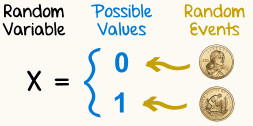
\includegraphics[width=2.5in]{rv.jpg}
\end{figure}
\FloatBarrier
}}

\begin{enumerate}
\easysubproblem{Here is a way to produce $X \sim \bernoulli{\half}$ using the $\Omega$ from a roll of a die. Map outcomes 1,2,3 to 0 and outcomes 4,5,6 to 1. This works because 

\beqn
&&\prob{X=0} = \prob{\braces{\omega : X(\omega) = 0}} = \prob{\braces{1, 2, 3}} = 1/2 ~~\text{and} \\ 
&&\prob{X=1} = \prob{\braces{\omega : X(\omega) = 1}} = \prob{\braces{4, 5, 6}} = 1/2.
\eeqn

Describe three other scenarios or devices that produce their own $\Omega$'s that also result in $X \sim \bernoulli{\half}.$ Be creative (i.e. not boring).} \spc{5}

\intermediatesubproblem{We talked about in class how the sample space no longer needs to be considered once the random variable is described. Why? Use your answer to (a) to inspire this answer. Write it \textit{in English} below.} \spc{3}

\hardsubproblem{Back to philosophy... Let's say $X$ models the price difference that IBM stock moves in one day of trading. For instance, if the stock closed yesterday at \$56.24 and today it closed at \$57.24, the random variable would be \$1 for today. According to our definition of a random variable, there is a sample space with outcomes being drawn ($\omega \in \Omega$) that is \qu{controlling} the value of $X$. Describe it the best you can \textit{in English}. There are no right or wrong answers here, but your answer must be coherent and demonstrate you understand the question.} \spc{6}

\end{enumerate}


\problem{We will now study probability mass functions (PMF's) denoted as $p(x)$ and cumulative distribution functions (CDF's) denoted as $F(X)$ and review the r.v.'s we did in class.}

\begin{enumerate}

\easysubproblem{Draw the PMF for $X \sim \bernoulli{p}$.}  \spc{3}

\easysubproblem{Draw the CDF for $X \sim \uniformdiscrete{1,3,4,9}$.}  \spc{3}

\intermediatesubproblem{Using the r.v. from the previous question, what is $\prob{X \in (3,9)}$? I am trying to trick you here.} \spc{3}

\hardsubproblem{In class we defined the Bernoulli r.v. as:

\beqn
X \sim \begin{cases}
1 \withprob p \\
0 \withprob 1-p
\end{cases}
\eeqn

and put its PMF on the board. Write $p(x)$ for $X \sim \bernoulli{p}$ that is only valid for not only all values in the $\support{X}$ but all values in $\reals$. Hint: use the indicator function.} \spc{1}

\easysubproblem{What is the parameter space of $X$ where $X \sim \bernoulli{p}$ and why?}  \spc{1.5}


%\hardsubproblem{Sometimes knowing the $\Omega$ matters a little bit. Let's say $X_1 \sim \bernoulli{\half}$ is generated from one coin and $X_2 \sim \bernoulli{\half}$ is generated from another coin independently tossed. Create a new r.v. $T = X_1 + X_2$. Describe its PMF using the $\sim$ notation like in the previous problem. Thus write \qu{$T \sim$} something.} \spc{13}

\hardsubproblem{Consider the PMF we discussed for $X \sim \bernoulli{\half}$. Does $\myint{x}{}{}{p(x)} = F(x) + C$ where the constant $C \in \reals$? Explain. Think carefully about what integration really means.} \spc{5}

\hardsubproblem{How about the opposite? Consider the CDF we discussed for $X \sim \bernoulli{\half}$. Does $\text{d} / \text{d}x[F(x)] = p(x)$? Explain. Think carefully about what differentiation really means.} \spc{3}


\end{enumerate}

\iftoggle{professormode}{
\paragraph{Hypergeometric Distribution} This is a very interesting random variable and we will cover it thoroughly between this homework and the next one.\\ \\
} 

\problem{The hypergeometric is sampling \qu{without replacement.} Imagine you have this bag of marbles with 37 marbles and 17 of them are black. We will define a \qu{success} as drawing a black marble.

\iftoggle{professormode}{
\begin{figure}[htp]
\centering
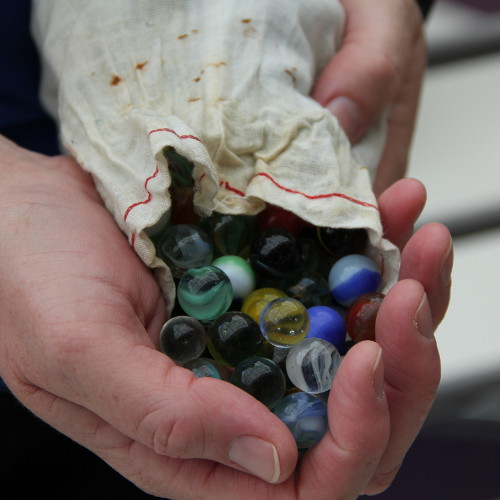
\includegraphics[width=2in]{marble.jpg}
\end{figure}
\FloatBarrier
}}

\begin{enumerate}

\easysubproblem{Let's say you draw one marble. Call this r.v. $X$. Is it hypergeometric?} \spc{0.2}

\easysubproblem{The hypergeometric distribution has three parameters. What are the parameters for $X$?} \spc{2}

\easysubproblem{Write, but do not draw, the PDF, $p(x)$ for the r.v. $X$ where $x$ is the number of successes.} \spc{2}

\easysubproblem{What is the support of this r.v.?} \spc{2}

\intermediatesubproblem{There is another variable we learned about in class with this same support. Show that $X$ is distributed as this type of r.v. and find its parameter(s).} \spc{2}

\easysubproblem{Now imagine you draw 4 marbles without replacement. Call this r.v. $X$ (and forget about the previous r.v. $X$ from this question, parts a-e). How is $X$ distributed? Use the notation in class and find its parameters.} \spc{2}

\easysubproblem{What is the support of $X$?} \spc{2}

\easysubproblem{Write, but do not draw, the PMF of $X$.} \spc{3}

\easysubproblem{Draw the PMF of $X$.} \spc{6}

\easysubproblem{Draw the CDF of $X$.} \spc{6}

\easysubproblem{What is the probability of getting 4 successes in a row? Use the PMF.} \spc{3}

%\easysubproblem{What is the probability of getting 4 successes in a row? Use conditional probability. This should yield the same answer.} \spc{3}

\easysubproblem{Now imagine you draw 27 marbles without replacement. Call this r.v. $X$ (and forget about the previous r.v. $X$). How is $X$ distributed? Use the notation in class and find its parameters.} \spc{2}

\easysubproblem{What is the support of $X$?} \spc{1}

\easysubproblem{Why is $0 \notin \support{X}$?} \spc{1}

\easysubproblem{Write, but do not draw, the PMF of $X$.} \spc{1}

\hardsubproblem{Find the mode of this distribution. \qu{Mode} is defined as the most likely outcome result.} \spc{6}

\end{enumerate}

\problem{Generally, the hypergeometric has three parameters. We will solve for its support here under several disjoint conditions and then in class we will generalize it. Call $X$ a hypergeometric r.v. with all its parameters free - meaning they can take on any value, so please use the notation $n,~K,~N$ in your answers as we did in class. This problem is just copying from your class notes.}

\begin{enumerate}
\easysubproblem{Using the usual parameterization of the hypergeometric, describe the parameter space. You need to say what sets each of the parameters \qu{lives} in. }\spc{4}

\easysubproblem{Write, but do not draw, the PMF of $X$. }\spc{3}

%\intermediatesubproblem{ $x$ is the free variable in $p(x)$ which you wrote in (b) and it designates the number of successes. Show that successes and failure are essentiall the same thing by finding $p(n-x)$ and replacing $K$ with $N-K$. What does this teach you? }\spc{2.5}

\easysubproblem{ Let's say $n < K$ and $n < N-K$. What is the support of $X$ in this situation? }\spc{3}

\easysubproblem{ Let's say $n < K$ and $n \geq N-K$. What is the support of $X$ in this situation? }\spc{3}

\easysubproblem{ Let's say $n \geq K$ and $n < N-K$. What is the support of $X$ in this situation? }\spc{3}
 
\easysubproblem{ Let's say $n \geq K$ and $n \geq N-K$. What is the support of $X$ in this situation? }\spc{2.5}

\intermediatesubproblem{Find a formula using a sum for the CDF of the general hypergeometric r.v. }\spc{6}


\extracreditsubproblem{Demonstrate that the sum of the PMF over the support is 1 (on a separate piece of paper).}\spc{11}

\end{enumerate}

%
%\problem{We will look at the general hypergeometric distribution with large $N$.}
%
%\begin{enumerate}
%
%\easysubproblem{We will now begin deriving the binomial in pieces. Parameterize a hypergeometric by setting $K = pN$. What is the parameter space for $p$? }\spc{2.5}
%
%\easysubproblem{Write the PMF $p(x)$ for this r.v. using the $p$ parameterization using $x$ as the free variable. }\spc{2.5}
%
%\easysubproblem{What limit do we take and why are we taking this limit? }\spc{2.5}
%
%\easysubproblem{Rewrite the PMF without choose notation using only factorials and simplify the fraction by moving the factorial terms from denominator, $\binom{N}{n}$, to the numerator.}
%
%\beqn
%p(x) = \lim_{N \rightarrow \infty} \frac{(pN)!}{\inpurple{x!} (pN - x)!} \frac{((1-p)N)!}{\inpurple{(n-x)!} ((1-p)N - n + x)!} \frac{\inpurple{n!} (N-n)!}{N!} 
%\eeqn
%
%\easysubproblem{Which three terms can you factor out from the limit expression? Show that they are equivalent to $\binom{n}{x}$. }\spc{5}
%
%
%\hardsubproblem{ Within the limit, you now have three ratios. Write these ratios by canceling out the common terms. For instance $10!/6! = 10 \times 9 \times 8 \times 7$ and $6!/10! = 1 / (10 \times 9 \times 8 \times 7)$. You have to get the indexing right.  }\spc{6}
%
%\intermediatesubproblem{ How many terms are in the numerator? How many terms are in the denominator.}
%
%There are $x$ terms in the first piece of the numerator and $n-x$ terms in the second piece of the denominator for a total of $n$ terms. Then there are $n$ terms in the denominator.
%
%\intermediatesubproblem{ Reason in English that the denominator looks like a bunch of $N - c_i$ where the $c_i$'s are all constants which are negligible as $N \rightarrow \infty$. }\spc{3}
%
%\intermediatesubproblem{ Reason in English that the numerator looks like a bunch of $Np - c_i$ where the $c_i$'s are all constants which are negligible as $N \rightarrow \infty$ as well as a bunch of $(1-p)N - c_i$ where the $c_i$'s are all constants which are negligible as $N \rightarrow \infty$.  }\spc{5}
%
%\intermediatesubproblem{ Match each $Np - c_i$ term in the numerator to one $N - c_i$ term in the denominator and take the limit of each one individually. Show that you wind up with $p \times p \times \ldots$ for a total of $x$ times, i.e. $p^x$. }\spc{4}
%
%\intermediatesubproblem{ Match each $(1-p)N - c_i$ term in the numerator to one $N - c_i$ term in the denominator and take the limit of each one individually. Show that you wind up with  $(1-p) \times (1-p) \times \ldots$ for a total of $n-x$ times, i.e. $ \tothepow{1-p}{n-x}$. }\spc{4}
%
%\easysubproblem{Using your answers from the previous parts to write the binomial r.v.'s PMF. }\spc{2}
%
%\extracreditsubproblem{ Imagine you are drawing $n$ successes with and without replacement. Derive a function of $N$ and $n$ which gives this percentage difference for $N$ and $n$ generally when the number of successes $K = \half N$. }\spc{7}
%
%
%\end{enumerate}


\problem{We will now look at the binomial in general.}

\begin{enumerate}

\intermediatesubproblem{ Show using the definition of equals in distribution that $X_1 \equalsindist X_2$ if $X_1 \sim \bernoulli{p}$ and $X_2 \sim \binomial{1}{p}$.  }\spc{3}

\intermediatesubproblem{Imagine an infinite bag where 47\% of the balls are \qu{successes}. If I draw 87 balls, what is the probability I get 29 success balls?}\spc{3}


\intermediatesubproblem{Imagine I have a bag with 300 balls where $141$ of the balls are \qu{successes}. If I draw 87 balls \textit{with replacement}, what is the probability I get 29 success balls?}\spc{3}


\intermediatesubproblem{Why is your answers to (c) and (d) the same?}\spc{3}

\easysubproblem{Let $\Xoneton \iid \bernoulli{p}$. Give a real-life example of this situation}\spc{4}

\easysubproblem{Let $T_n = X_1 + \ldots + X_n$ where $\Xoneton \iid \bernoulli{p}$. How is $T_n$ distributed? }\spc{1}

\hardsubproblem{Let $X_1, \ldots, X_n \iid \bernoulli{p}$ and $T_n = \sum_{i=1}^n X_i$. Derive the distribution of $T_n$ from first principles just like we did in the notes.}\spc{11}

\end{enumerate}


\problem{Imagine two Bernoulli r.v.'s $X_1$ and $X_2$ which model two fair coin flips where Heads is mapped to 1 and tails is mapped to 0. The probability of heads is 1/2.}

\begin{enumerate}

\easysubproblem{Given no other information, explain using the definition of r.v. independence why these two r.v.'s are independent. }\spc{2}

\easysubproblem{Given no other information, explain using the definition of equality in distribution why $X_1 \equalsindist X_2$. }\spc{2}

\easysubproblem{Are $X_1, X_2 \iid \bernoulli{p}$? }\spc{1}

\intermediatesubproblem{ Now imagine these two coins were linked using some sort of sorcery. They are flipped at the same time but are guaranteed to flip the same way. That is, if the first coin goes heads, the second coin must go heads (and if the first coin goes tails, the second coin must go tails).

\iftoggle{professormode}{
\begin{figure}[htp]
\centering
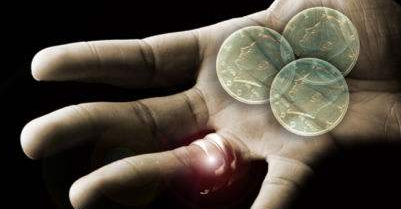
\includegraphics[width=2.8in]{magiccoins.png}
\end{figure}
\FloatBarrier
}

Explain using the definition of r.v. independence why these two r.v.'s are \textit{dependent}.}\spc{4}


\hardsubproblem{ Using the same two sorcery-controlled coins, explain using the definition of equality in distribution why or why not $X_1 \equalsindist X_2$. }\spc{3}



\easysubproblem{Let $T_2 = X_1 + X_2$. Is $T_2 \sim \binomial{2}{\half}$? Why or why not?  }\spc{4}

\end{enumerate}


\end{document}




